% Drawing angles using the PG 3.0 angles and quotes libraries

\documentclass[tikz,border=10pt]{standalone}
\usetikzlibrary{quotes,angles}

\begin{document}
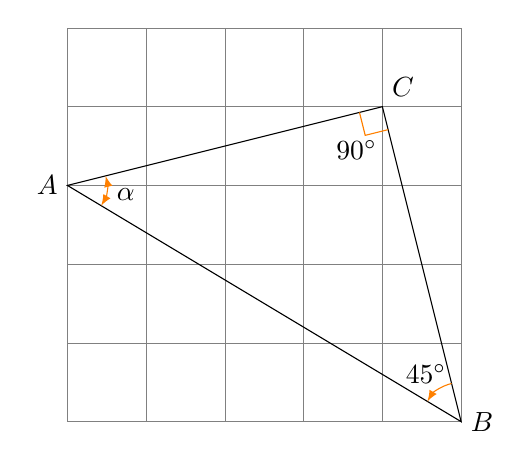
\begin{tikzpicture}
  \draw[help lines] (0,0) grid (5,5);
  \draw
    (0,3) coordinate (A) node[left] {$A$}
    -- (4,4) coordinate (C) node[above right] {$C$}
    -- (5,0) coordinate (B) node[right] {$B$} -- cycle;

  \draw pic["$\alpha$", draw=orange, latex-latex, angle eccentricity=1.5, angle radius=5mm]
    {angle=B--A--C};
  \draw pic["$45^\circ$", draw=orange, -latex, angle eccentricity=1.5, angle radius=5mm]
    {angle=C--B--A};
  \draw pic["$90^\circ$", draw=orange, angle eccentricity=1.5, angle radius=3mm]
    {right angle=A--C--B};
\end{tikzpicture}
\end{document}